\exercisesection

\begin{exercise} \label{exercise 5.4.1}
Label the following statements as true or false.
\begin{enumerate}
\item There exists a linear operator \(\T\) with no \(\T\)-invariant subspace.
\item If \(\T\) is a linear operator on a finite-dimensional vector space \(\V\) and \(\W\) is a \(\T\)-invariant subspace of \(\V\), then the \CPOLY{} of \(\T_W\) divides the \CPOLY{} of \(\T\).
\item Let \(\T\) be a linear operator on a finite-dimensional vector space \(\V\), and let \(v\) and \(w\) be in \(\V\).
If \(\W\) is the \(\T\)-cyclic subspace generated by \(v\), \(\W'\) is the \(\T\)-cyclic subspace generated by \(w\), and \(\W = \W'\), then \(v = w\).
\item If \(\T\) is a linear operator on a finite-dimensional vector space \(\V\), then for any \(v \in \V\) the \(\T\)-cyclic subspace generated by \(v\) is the same as the \(\T\)-cyclic subspace generated by \(\T(v)\).
\item Let \(\T\) be a linear operator on an \(n\)-dimensional vector space.
Then there exists a polynomial \(g(t)\) of degree \(n\) such that \(g(\T) = \TZERO\).
\item Any polynomial of degree \(n\) with leading coefficient \((-1)^n\) is the \CPOLY{} of some linear operator.
\item If \(\T\) is a linear operator on a finite-dimensional vector space \(\V\), and if \(\V\) is the direct sum of \(k\) \(\T\)-invariant subspaces, then there is an ordered basis \(\beta\) for \(\V\) such that \([\T]_{\beta}\) is a direct sum of \(k\) \emph{matrices}.
\end{enumerate}
\end{exercise}

\begin{proof} \ 

\begin{enumerate}
\item False. Every linear operator has \(\{ \OV \}\) and \(\V\) as (trivial) invariant subspaces.
\item True by \THM{5.20}.
\item False.
From \EXAMPLE{5.4.3}, let \(v = e_1, w = e_2\), then from that example \(\W = \W' = \spann(\{ e_1, e_2 \})\), but \(v \ne w\).

\item False. Let \(\V = \POLYRRR\) and \(\T(f(x)) = f'(x)\).
Let \(v = x^3\), then the \(\T\)-cyclic subspace generated by \(v\) is \(\spann(\{ x^3, 3x^2, 6x, 6, 0, ... \}) = \POLYRRR\), but the \(\T\)-cyclic subspace generated by \(\T(v)\) is \(\spann(\{ 3x^2, 6x, 6, 0, ... \}) = \POLYRR \ne \POLYRRR\).
\item True; The \CPOLY{} of any linear operator is degree \(n\), and \(\T\) ``satisfies'' its \CPOLY{} by \THM{5.22}.
\item By \EXEC{5.4.19}, any \(n \X n\) matrix \(A\) with the form given in that exercise has \CPOLY{} with \((-1)^n\) as the leading coefficient, and that matrix corresponding to a linear operator.
\item True by \THM{5.24}.
\end{enumerate}
\end{proof}

\begin{exercise} \label{exercise 5.4.2}
For each of the following linear operators \(\T\) on the vector space \V, determine whether the given subspace \(\W\) is a \(\T\)-invariant subspace of \(v\).
\begin{enumerate}
\item \(\V = \POLYRRR\), \(\T(f(x)) = f'(x)\), and \(\W = \POLYRR\)
\item \(\V = \POLYRINF\), \(\T(f(x)) = x \cdot f(x)\), and \(\W = \POLYRR\)
\item \(\V = \SET{R}^3\), \(\T(a, b, c) = (a + b + c, a + b + c, a + b + c)\), and \(\W = \{ (t, t, t): t \in \SET{R} \}\)
\item \(\V = \mathcal{C}([0, 1])\), \(\T(f(t)) = [\int_0^1 f(x) dx]t\), and \(\W = \{f \in \V: f(t) = at + b \text{ for some \(a\) and \(b\)} \}\)
\item \(\V = M_{2 \X 2}(\SET{R})\), \(\T(A) = \begin{pmatrix} 0 & 1 \\ 1 & 0 \end{pmatrix} A\), and \(\W = \{A \in \V: A^\top = A \}\)
\end{enumerate}
\end{exercise}

\begin{proof} \ 

\begin{enumerate}
\item Of course! Given \(f(x) \in \POLYRR\) with degree \(\le 2\), the output, \(\T(f(x)) = f'(x)\), has degree \(\le 1\), so by definition is still in \(\POLYRR\).

\item \(\W = \POLYRR\) is not a \(\T\)-invariant subspace: Given \(x^2 \in \POLYRR\), \(\T(x^2) = x \cdot x^2 = x^3\), which by definition is not in \(\POLYRR\).

\item Given any \((t, t, t) \in \W\) where \(t \in \SET{R}\), \(\T(t, t, t) = (t + t + t, t + t + t, t + t + t) = (3t, 3t, 3t)\), which by definition is in \(\W\) since \(3t \in \SET{R}\).
Hence \(\W\) is a \(\T\)-invariant subspace.

\item Given any \(f(t) \in \W\), without loss of generality let \(f(t) = at + b\) for some \(a\) and \(b\).
Then
\begin{align*}
    \T(at + b) = \left[ \int_0^1 ax + b dx \right] \cdot t
    & = \left[ \frac{a}{2} x^2 + bx \Big|_0^1 \right] \cdot t \\
    & = \left[ \frac{a}{2} + b - (0 + 0) \right] \cdot t \\
    & = \left[ \frac{a}{2} + b \right] \cdot t \\
    & = \left[ \frac{a}{2} + b \right] \cdot t + 0 = a't + b',
\end{align*}
where \(a' = \frac{a}{2} + b\) and \(b' = 0\), hence \(a't + b'\) is still in \(\W\).
So \(\W\) is a \(\T\)-invariant subspace.

\item Given \(A \in \W\), without loss of generality let \(A = \begin{pmatrix} a & b \\ b & c \end{pmatrix}\).
Then
\begin{align*}
    \T(A) = \T \begin{pmatrix} a & b \\ b & c \end{pmatrix}
          = \begin{pmatrix} 0 & 1 \\ 1 & 0 \end{pmatrix} \begin{pmatrix} a & b \\ b & c \end{pmatrix}
          = \begin{pmatrix} b & c \\ a & b \end{pmatrix}
\end{align*}
which is not necessarily symmetric, hence is not necessarily in \(\W\).
Hence \(\W\) is not a \(\T\)-invariant subspace.
\end{enumerate}
\end{proof}

\begin{exercise} \label{exercise 5.4.3}
Let \(\T\) be a linear operator on a finite-dimensional vector space \(\V\).
Prove that the following subspaces are \(\T\)-invariant.
\begin{enumerate}
\item \(\{ \OV \}\) and \(\V\)
\item \(\NULLT\) and \(\RANGET\)
\item \(E_{\lambda}\) for any eigenvalue \(\lambda\) of \(\T\)
\end{enumerate}
\end{exercise}

\begin{proof}
For (a) and (b), see \EXEC{2.1.29}.

For part(c), let \(\lambda\) be an arbitrary eigenvalue of \(\T\), an arbitrary linear operator.
Now let \(v \in E_{\lambda}\); then by definition, \(\T(v) = \lambda v\).
But \(\T(\T(v)) = \T(\lambda v) = \lambda \T(v) = \lambda (\lambda v) = \lambda \T(v)\).
Hence by definition \(\T(v) \in E_{\lambda}\).
So \(E_{\lambda}\) is a \(\T\)-invariant subspace.
\end{proof}

\begin{exercise} \label{exercise 5.4.4}
Let \(\T\) be a linear operator on a vector space \(\V\), and let \(\W\) be a \(\T\)-invariant subspace of \(\V\).
Prove that \(\W\) is \(g(\T)\)-invariant for any polynomial \(g(t)\).
\end{exercise}

\begin{proof}
Without loss of generality let \(g(t) = a_0 + a_1 t + ... + a_k t^k\).
Then given \(v \in \W\),
\begin{align*}
    g(\T)(v) & = (a_0 \ITRANV{} + a_1 \T + ... + a_k \T^k)(v) & \text{by \DEF{e.3}} \\
        & = a_0 \ITRANV{}(v) = a_1 \T(v) + ... + a_k \T^k(v) & \text{since function \(+, \cdot\) is linear}
\end{align*}
Furthermore, by definition of invariant subspace and induction, we have \(\T^k(v) \in \W\) for any nonnegative integer \(k\) and \(v \in \W\).
Hence \(g(\T(v)) = a_0 \ITRANV{}(v) = a_1 \T(v) + ... + a_k \T^k(v)\) is a linear combination of elements in \(\W\), hence is still in \(\W\).
So \(\W\) is a \(g(\T)\)-invariant subspace.
\end{proof}

\begin{exercise} \label{exercise 5.4.5}
Let \(\T\) be a linear operator on a vector space \(\V\).
Prove that the \emph{intersection} of any collection of \(\T\)-invariant subspaces of \(\V\) is a \(\T\)-invariant subspace of \(\V\).
\end{exercise}

\begin{proof}
Let \(\W_{\alpha}\) be a collection of \(\T\)-invariant subspaces of \(\V\) where \(\alpha \in \Lambda\).
Now \textbf{let} \(v \in \bigcap_{\alpha \in \Lambda} \W_{\alpha}\).
First, (by \THM{1.4}) the intersection of subspaces is also a subspace.
Then \(v \in \W_{\alpha}\) for all \(\alpha \in \Lambda\).
Furthermore, \(\T(v) \in \W_{\alpha}\) for all \(\alpha \in \Lambda\).
\textbf{Hence} \(\T(v) \in \bigcap_{\alpha \in \Lambda} \W_{\alpha}\).
So \(\bigcap_{\alpha \in \Lambda} \W_{\alpha}\) is a \(\T\)-invariant subspace of \(\V\).
\end{proof}

\begin{exercise} \label{exercise 5.4.6}
For each linear operator \(\T\) on the vector space \(\V\), find an ordered basis for the \(\T\)-cyclic subspace generated by the vector \(z\).
\begin{enumerate}
\item \(\V = \SET{R}^4\), \(\T(a, b, c, d) = (a + b, b - c, a + c, a + d)\), and \(z = e_1\).
\item \(\V = \POLYRRR\), \(\T(f(x)) = f''(x)\), and \(z = x^3\).
\item \(\V = M_{2 \X 2}(\SET{R})\), \(\T(A) = A^\top\), and \(z = \begin{pmatrix} 0 & 1 \\ 1 & 0 \end{pmatrix}\)
\item \(\V = M_{2 \X 2}(\SET{R})\), \(\T(A) = \begin{pmatrix} 1 & 1 \\ 2 & 2 \end{pmatrix} A\), and \(z = \begin{pmatrix} 0 & 1 \\ 1 & 0 \end{pmatrix}\)
\end{enumerate}
\end{exercise}

\begin{proof}
We use the steps in the proof of \THM{5.21}(a).
\begin{enumerate}
\item
\begin{align*}
    \T(e_1) & = \T(1, 0, 0, 0) = (1, 0, 1, 1) \\
    \T^2(e_1) & = \T(\T(e_1)) = \T(1, 0, 1, 1) = (1, -1, 2, 2) \\
    \T^3(e_1) & = \T(\T^2(e_1)) = \T(1, -1, 2, 2) = (0, -3, 3, 3)
\end{align*}
\sloppy Note that \((0, -3, 3, 3) = 3(1, -1, 2, 2) - 3(1, 0, 1, 1)\), so \(\{ e_1, \T(e_1), \T^2(e_1), \T^3(e_1) \}\) is \LDP{} but \(\{ e_1, \T(e_1), \T^2(e_1)\}\) is \LID{}.
Hence \(\{ e_1, \T(e_1), \T^2(e_1) \} = \{ (1, 0, 0, 0), (1, 0, 1, 1), (1, -1, 2, 2) \}\) is an ordered basis for the \(\T\)-cyclic subspace generated by \(e_1\).

\item
\begin{align*}
    \T(x^3) & = (x^3)'' = 6x \\
    \T^2(x^3) & = \T(\T(x^3)) = \T(6x) = (6x)'' = 0,
\end{align*}
Note that \(\{ x^3, 6x, 0 \}\) is \LDP{} but \(\{ x^3, 6x \}\) is \LID{}.
Hence \(\{ x^3, \T(x^3) \} = \{ x^3, 6x \}\) is an ordered basis for the \(\T\)-cyclic subspace generated by \(x^3\).

\item
\begin{align*}
    \T(z) = \T \begin{pmatrix} 0 & 1 \\ 1 & 0 \end{pmatrix} = \begin{pmatrix} 0 & 1 \\ 1 & 0 \end{pmatrix}^\top = \begin{pmatrix} 0 & 1 \\ 1 & 0 \end{pmatrix}.
\end{align*}
So \(z = \T(z)\), hence \(\{ z, \T(z) \}\) is \LDP{}, but the singleton set \(\{ z \}\) is not.
Hence \(\{ z \} = \left\{ \begin{pmatrix} 0 & 1 \\ 1 & 0 \end{pmatrix} \right\}\) is an ordered basis for the \(\T\)-cyclic subspace generated by \(\begin{pmatrix} 0 & 1 \\ 1 & 0 \end{pmatrix}\).

\item
\begin{align*}
    \T(z) & = \T \begin{pmatrix} 0 & 1 \\ 1 & 0 \end{pmatrix} = \begin{pmatrix} 1 & 1 \\ 2 & 2 \end{pmatrix} \begin{pmatrix} 0 & 1 \\ 1 & 0 \end{pmatrix} = \begin{pmatrix} 1 & 1 \\ 2 & 2 \end{pmatrix}, \\
    \T^2(z) & = \T(\T(z)) = \T \begin{pmatrix} 1 & 1 \\ 2 & 2 \end{pmatrix} = \begin{pmatrix} 1 & 1 \\ 2 & 2 \end{pmatrix} \begin{pmatrix} 1 & 1 \\ 2 & 2 \end{pmatrix} = \begin{pmatrix} 3 & 3 \\ 6 & 6 \end{pmatrix} = 3 \begin{pmatrix} 1 & 1 \\ 2 & 2 \end{pmatrix}
\end{align*}
So \(\{ z, \T(z), \T^(z) \}\) is \LDP{} but \(\{ z, \T(z) \}\) is not.

Hence \(\{ z, \T(z) \} = \left\{ \begin{pmatrix} 0 & 1 \\ 1 & 0 \end{pmatrix}, \begin{pmatrix} 1 & 1 \\ 2 & 2 \end{pmatrix} \right\}\) is an ordered basis for the \(\T\)-cyclic subspace generated by \(\begin{pmatrix} 0 & 1 \\ 1 & 0 \end{pmatrix}\).
\end{enumerate}
\end{proof}

\begin{exercise} \label{exercise 5.4.7}
Prove that the restriction of a linear operator \(\T\) to a \(\T\)-invariant subspace is a linear operator on that subspace.
\end{exercise}

\begin{proof}
See \EXEC{2.1.30}.
\end{proof}

\begin{exercise} \label{exercise 5.4.8}
Let \(\T\) be a linear operator on a vector space with a \(\T\)-invariant subspace \(\W\).
Prove that if \(v\) is an eigenvector \textbf{of \(\T_W\)} with corresponding eigenvalue \(\lambda\), then \(v\) is also an eigenvector \textbf{of \(\T\)} with corresponding eigenvalue \(\lambda\).
\end{exercise}

\begin{proof}
Suppose \(v\) is an eigenvector of \(\T_W\) with corresponding eigenvalue \(\lambda\), where \(\W\) is a \(\T\)-invariant subspace.
(In particular, of course \(v \in \W\).)
Then
\begin{align*}
    \T(v) & = \T_W(v) & \text{since \(v \in \W\)} \\
          & = \lambda v & \text{since \(v\) is an e.v. of \(\T_W\) corresponding to \(\lambda\)}
\end{align*}
Then by definition \(v\) is an eigenvector of \(\T\) with corresponding eigenvalue \(\lambda\).
\end{proof}

\begin{exercise} \label{exercise 5.4.9}
For each linear operator \(\T\) and cyclic subspace \(\W\) in \EXEC{5.4.6}, compute the \CPOLY{} of \(\T_W\) in two ways, as in \EXAMPLE{5.4.6}.
\end{exercise}

\begin{proof}
(Please refer to \EXEC{5.4.6}.)
Skip the second way, computing by determinants.
\begin{enumerate}
\item We already have \((0, -3, 3, 3) = 3(1, -1, 2, 2) - 3(1, 0, 1, 1)\), or \(\T^3(e_1) = 3\T^2(e_1) - 3\T(e_1)\).
In particular, we have
\[
    0 e_1 + 3\T(e_1) - 3\T^2(e_1) + \T^3(e_1) = \OV.
\]
So by \THM{5.21}(b), the \CPOLY{} of \(\T_W\) is \((-1)^3(0 + 3t - 3t^2 + t^3) = -t^3 + 3t^2 - 3t\).

\item We already have \(\T^2(x^3) = 0\), in particular,
\[
    0 x^3 + 0 \T(x^3) + \T^2(x^3) = 0.
\]
So by \THM{5.21}(b), the \CPOLY{} of \(\T_W\) is \((-1)^2(0 + 0t + t^2) = t^2\).

\item We already have \(z = \T(z)\), in particular,
\[
    -1 z + \T(z) = O_{2 \X 2}.
\]
So by \THM{5.21}(b), the \CPOLY{} of \(\T_W\) is \((-1)^1(-1 + t) = 1 - t\).

\item We already have \(\T^2(z) = 3\T(z)\), in particular,
\[
    0 z - 3\T(z) + \T^2(x) = O_{2 \X 2}.
\]
So by \THM{5.21}(b), the \CPOLY{} of \(\T_W\) is \((-1)^2(0 - 3t + t^2) = t^2 - 3t\).
\end{enumerate}
\end{proof}

\begin{exercise} \label{exercise 5.4.10}
For each linear operator in \EXEC{5.4.6}, find the \CPOLY{} \(f(t)\) of \(\T\), and verify that the \CPOLY{} of \(\T_W\) (computed in \EXEC{5.4.9}) divides \(f(t)\).
\end{exercise}

\begin{proof}
Skip.
\end{proof}

\begin{exercise} \label{exercise 5.4.11}
Let \(\T\) be a linear operator on a vector space \(\V\), let \(v\) be a nonzero vector in \(\V\), and let \(\W\) be the \(\T\)-cyclic subspace of \(\V\) generated by \(v\).
Prove that
\begin{enumerate}
\item \(\W\) is \(\T\)-invariant.
\item Any \(\T\)-invariant subspace of \(\V\) containing \(v\) also contains \(\W\).
\end{enumerate}
\end{exercise}

\begin{proof} \ 

\begin{enumerate}
\item Suppose arbitrary \(w \in \W\).
Then without loss of generality, \(w = a_0 v + a_1 \T(v) + ... + a_k \T^k(v)\) for some positive integer \(k\), where some \(a_i\) can be zero.
Hence
\begin{align*}
    \T(w) & = \T(a_0 v + a_1 \T(v) + ... + a_k \T^k(v)) \\
          & = a_0 \T(v) + a_1 \T(\T(v)) + ... + a_k \T(\T^k(v)) & \text{since \(\T\) is linear} \\
          & = a_0 \T(v) + a_1 \T^2(v) + ... + a_k \T^{k + 1}(v),
\end{align*}
which by definition is in \(\W\).
Hence \(\W\) is \(\T\)-invariant subspace of \(\V\).

\item Suppose \(\W'\) is a \(\T\)-invariant subspace containing \(v\).
And suppose arbitrary \(w \in \W\); we have to show \(w \in \W'\).
Again, without loss of generality, \(w = a_0 v + a_1 \T(v) + ... + a_k \T^k(v)\) for some positive integer \(k\), where some \(a_i\) can be zero.
Since \(v \in \W'\) and \(\W'\) is \(\T\)-invariant subspace, (by definition of invariant subspace and induction,) we have \(c \T^i(v) \in \W'\) for any scalar \(c\) and positive integer \(i\), therefore, any linear combination of \(a_i \T^i(v)\)'s is in \(\W\).
Hence \(w \in \W'\), as desired.
\end{enumerate}
\end{proof}

\begin{exercise} \label{exercise 5.4.12}
Prove that \(A = \begin{pmatrix} B_1 & B_2 \\ O & B_3 \end{pmatrix}\) in the proof of \THM{5.20}.
\end{exercise}

\begin{proof}
(Let \(\T, \W, \gamma, \beta, A, B_1\) be as in the proof of \THM{5.20}.)
Note that for \(v \in \gamma\)
\[
    \T(v) = \T_W(v) \in W,
\]
which means that \(\T(v) \in \W\) and can be written as linear combination of elements in \(\gamma\).
Specifically, that means
\[
    \T(v) = \sum_{i = 1}^{\RED{n}} a_i v_i = \sum_{i=1}^{\RED{k}} a_i v_i
\]
which means that first \(k\) columns of \(A\) have zeros on last \(n - k\) entries.
And since \(\T(v) = \T_W(v)\), then the first \(k\) entries of the first \(k\) columns of \(A\) are exactly the same as \([\T_W]_{\gamma}\), that is, \(B_1\).
\end{proof}

\begin{exercise} \label{exercise 5.4.13}
Let \(\T\) be a linear operator on a vector space \(\V\), let \(v\) be a nonzero vector in \(\V\), and let \(\W\) be the \(\T\)-cyclic subspace of \(\V\) generated by \(v\).
For any \(w \in \V\), prove that \(w \in \W\) if and only if there exists a polynomial \(g(t)\) such that \(w = g(\T)(v)\).
\end{exercise}

\begin{note}
We do \emph{not} say that \(\V\) is finite-dimensional.
In particular, \THM{5.21} does \emph{not} apply.
\end{note}

\begin{proof}
\(w \in \W\), if and only if \(w = a_0 v + a_1 \T(v) + ... + a_k \T^k(v)\) for some \(a_i\) and positive integer \(k\),
if and only if \(w = (a_0 \ITRANV{} + a_1 \T + ... + a_k \T^k)(v)\), if and only if \(w = g(\T)(v)\) where \(g(t) = a_0 + a_1 t + ... + a_k t^k\).
\end{proof}

\begin{exercise} \label{exercise 5.4.14}
Prove that the polynomial \(g(t)\) of \EXEC{5.4.13} can always be chosen so that its degree is less than \(\dim(\W)\).
\end{exercise}

\begin{proof}
Let \(k = \dim(\W)\), then by \THM{5.21}, we have \(\beta = \{ v, \T(v), ..., \T^{k - 1}(v) \}\) is a basis for \(\W\).
So any \(w \in \W\) can be represented as a linear combination \(a_0 v + a_1 \T(v) + ... + a_k \T^{k - 1}(v)\), which can be represented as \(g(\T)(v)\) where \(g(t) = a_0 + a_1 t + ... + a_k t^{k - 1}\), which has degree less than \(k = \dim(\W)\).
\end{proof}

\begin{exercise} \label{exercise 5.4.15}
Use the Cayley-Hamilton theorem (\THM{5.22}) to prove its corollary, \CORO{5.22.1}, for matrices.
\RED{Warning}: If \(f(t) = \det(A - tI)\) is the \CPOLY{} of \(A\), it is tempting to ``prove'' that \(f(A) = O\) by saying ``\(f(A) = \det(A - AI) = \det(O) = 0\).''
Why is this argument incorrect?
\end{exercise}

\begin{proof}
See \CORO{5.22.1}.

Why the argument is incorrect? The argument says \(f(A)\), a (linear combination of a) matrix, turns out to be equal to \(0\), a scalar, which does not make sense.
\end{proof}

\begin{exercise} \label{exercise 5.4.16}
Let \(\T\) be a linear operator on a finite-dimensional vector space \(\V\).
\begin{enumerate}
\item Prove that if the \CPOLY{} of \(\T\) splits, then so does the \CPOLY{} of the restriction of \(\T\) to any \(\T\)-invariant subspace of \(\V\).
\item Deduce that if the \CPOLY{} of \(\T\) splits, then any nontrivial \(\T\)-invariant subspace of \(\V\) contains an eigenvector of \(\T\).
\end{enumerate}
\end{exercise}

\begin{proof}
I assume that the ``trivial'' invariant subspaces means \(\{ \OV \}\).
\begin{enumerate}
\item We prove the contrapositive of the statement.
Let \(f(t)\) be the \CPOLY{} of \(\T\).
Suppose there exists a \(\T\)-invariant subspace \(\W\) of \(\V\) such that the \CPOLY{}, \(g(t)\), of \(\T_W\) does not split.
Then by \THM{5.20}, \(g(t)\) divides \(f(t)\), which implies \(f(t)\) does not split since \(f(t)\) has a factor which does not split.

\item Suppose \(\W\) is any \emph{nontrivial} \(\T\)-invariant subspace.
So \(\W\) has dimensional greater than or equal to \(1\).
So the \CPOLY{}, \(g(t)\), of \(\T_W\) has degree greater than or equal to \(1\).
And by part(a), \(g(t)\) splits.
So \(g(t)\) splits and has degree greater than or equal to \(1\), which implies it must have at least one zero.
So \(\T_W\) has at least one eigenvalue \(\lambda\), hence has an eigenvector \(v\) in \(\W\).
But by \EXEC{5.4.8}, \(\lambda\) is an eigenvalue of \(\T\), hence \(v\) is an eigenvector of \(\T\) in \(\W\), as desired.
\end{enumerate}
\end{proof}

\begin{exercise} \label{exercise 5.4.17}
Let \(A\) be an \(n \X n\) matrix.
Prove that
\[
    \dim(\spann(\{ I_n, A, A^2, ... \})) \le n.
\]
\end{exercise}

\begin{note}
That span is a subspace of \(M_{n \X n}(F)\), which have \emph{finite} dimension \(n^2\).
The exercise shows that the ``cyclic'' subspace ``generated'' by any matrix, only has dimension at most \(n\).
\end{note}

\begin{proof}
Let \(f(t)\) be the \CPOLY{} of \(A\), such that
\[
    f(t) = (-1)^n t^n + a_{n - 1} t^{n - 1} + ... + a_1 t + a_0.
\]
(where the leading coefficient \((-1)^n\) is guaranteed by \THM{5.3}(a).)
By \THM{5.22}, Cayley-Hamilton, we have
\[
    f(A) = (-1)^n A^n + a_{n - 1} A^{n - 1} + ... + a_1 A + a_0 I = O_{n \X n}.
\]
This means \(A^n\) is a linear combination of \(I, A, A^2, ..., A^{n - 1}\). \MAROON{(1)}

Multiplying by \(A\), we have
\[
    (-1)^n A^{n + 1} + a_{n - 1} A^{n} + ... + a_1 A^2 + a_0 A = O_{n \X n} A = O.
\]
This means \(A^{n + 1}\) is a linear combination of \(A, A^2, ..., A^{n - 1}, A^{\RED{n}}\). \MAROON{(2)}

But with \MAROON{(1)}, the \(A^{\RED{n}}\) in \MAROON{(2)} can be represented only using \(I, A, A^2, ..., A^{n - 1}\), so they just imply \(A^{n + 1}\) is also a linear combination of \(I, A, A^2, ..., A^{\RED{n - 1}}\).
\emph{Inductively}, we have \(A^k\) can be represented \emph{only} using \(I, A, A^2, ..., A^{\RED{n - 1}}\), for any positive integer \(k\).
Hence \(\spann(\{ I, A, A^2, ... \}) = \spann(\{ I, A, A^2, ..., A^{n - 1}\})\), and the right side has dimension less than or equal to \(n\), hence
\[
    \dim(\spann(\{ I_n, A, A^2, ... \})) \le n,
\]
as desired.
\end{proof}

\begin{exercise} \label{exercise 5.4.18}
Let \(A\) be an \(n \X n\) matrix with \CPOLY{}
\[
    f(t) = (-1)^n t^n + a_{n - 1} t^{n - 1} + ... + a_1 t + a_0.
\]
\begin{enumerate}
\item Prove that \(A\) is invertible if and only if \(a_0 \ne 0\).
\item Prove that if \(A\) is invertible, then
\[
    A^{-1} = \frac{-1}{a_0} [(-1)^n A^{n - 1} + a_{n - 1} A^{n - 2} + ... + a_1 I_n].
\]
\item Use (b) to compute \(A^{-1}\) for
\[
    A = \begin{pmatrix} 1 & 2 & 1 \\ 0 & 2 & 3 \\ 0 & 0 & -1 \end{pmatrix}.
\]
\end{enumerate}
\end{exercise}

\begin{proof} \ 

\begin{enumerate}
\item This was proved in \EXEC{5.1.20}.
\item Suppose \(A\) is invertible, hence by part(a), the \(a_0\) in \(f(t)\) defined above is nonzero.
And by \THM{5.22}, \(f(A) = O_{n \X n}\), that is,
\[
    (-1)^n A^n + a_{n - 1} A^{n - 1} + ... + a_1 A + a_0 I = O_{n \X n}.
\]
And by calculation,
\begin{align*}
             & -a_0 I = (-1)^n A^n + a_{n - 1} A^{n - 1} + ... + a_1 A \\
    \implies & -a_0 I A^{-1} = ((-1)^n A^n + a_{n - 1} A^{n - 1} + ... + a_1 A) A^{-1} \\
             & \quad \quad \text{(by multiplying \(A^{-1}\))} \\
    \implies & -a_0 A^{-1} = (-1)^n A^n A^{-1} + a_{n - 1} A^{n - 1} A^{-1} + ... + a_2 A^2 A^{-1} + a_1 A A^{-1} \\
    \implies & -a_0 A^{-1} = (-1)^n A^{n - 1} + a_{n - 1} A^{n - 2} + ... + a_2 A + a_1 \\
    \implies & A^{-1} = -\frac{1}{a_0} \left[ (-1)^n A^{n - 1} + a_{n - 1} A^{n - 2} + ... + a_2 A + a_1 \right]
\end{align*}

\item 
By calculation,
\[
    f(t) = -t^3 + 2t^2 + t - 2.
\]
Hence by part(b),
\begin{align*}
    A^{-1} & = -\frac{1}{-2} ( (-1)^3 A^2 + 2 A^1 + 1 I ) \\
           & = \frac{1}{2} (-A^2 + 2 A + I) \\
           & = \frac{1}{2} \left(
               - \begin{pmatrix} 1 & 6 & 6 \\ 0 & 4 & 3 \\ 0 & 0 & 1 \end{pmatrix}
               + 2 \begin{pmatrix} 1 & 2 & 1 \\ 0 & 2 & 3 \\ 0 & 0 & -1 \end{pmatrix}
               + \begin{pmatrix} 1 & 0 & 0 \\ 0 & 1 & 0 \\ 0 & 0 & 1 \end{pmatrix}
           \right) \\
           & = \begin{pmatrix}
               0 & -1 & -2 \\
               0 & 0.5 & 1.5 \\
               0 & 0 & -1
           \end{pmatrix}.
\end{align*}
\end{enumerate}
\end{proof}

\begin{exercise} \label{exercise 5.4.19}
Let \(A\) denote the \(k \X k\) matrix
\[
    \begin{pmatrix}
        0      & 0      & \dots  & 0 & -a_0 \\
        1      & 0      & \dots  & 0 & -a_1 \\
        0      & 1      & \dots  & 0 & -a_2 \\
        \vdots & \vdots & \ddots & 0 & \vdots \\
        0      & 0      & \dots  & 1 & -a_{k - 1}
    \end{pmatrix},
\]
where \(a_0, a_1, ..., a_{k - 1}\) are arbitrary scalars.
Prove that the \CPOLY{} of \(A\) is
\[
    (-1)^k (t^k + a_{k - 1} t^{k-1} + ... + a_1 t + a_0).
\]
\emph{Hint}: Use mathematical induction on \(k\), computing the determinant by cofactor expansion along the first row.
\end{exercise}

\begin{proof}
For \(k = 1\), we have \(A = (-a_0)\), and the \CPOLY{} of \(A\) is
\begin{align*}
    \det \begin{pmatrix} -a_0 - t \end{pmatrix}
    & = (-a_0 - t) & \text{of course by definition} \\
    & = (-1)^1 (t^1 + a_0) & \text{of course} \\
\end{align*}
so the statement is true for \(k = 1\).

Suppose inductively that the statement is true for \(A \in M_{(k - 1) \X (k - 1)}(F)\) where \(k > 1\).
We have to show the statement is true for \(A \in M_{k \X k}(F)\).
Then the \CPOLY{} of \(A\) is
\begin{align*}
    & \det(A - tI) \\
    & = \begin{pmatrix}
        -t     & 0      & \dots  & 0 & -a_0 \\
        1      & -t     & \dots  & 0 & -a_1 \\
        0      & 1      & \dots  & 0 & -a_2 \\
        \vdots & \vdots & \ddots & 0 & \vdots \\
        0      & 0      & \dots  & 1 & -a_{k - 1} - t
    \end{pmatrix} \\
    & = (-t) \cdot (-1)^{1 + 1} \cdot \det \begin{pmatrix}
        & -t     & \dots  & 0 & -a_1 \\
        & 1      & \dots  & 0 & -a_2 \\
        & \vdots & \ddots & 0 & \vdots \\
        & 0      & \dots & 1 & -a_{k - 1}-t
    \end{pmatrix}
      + (-a_0) \cdot (-1)^{1 + k} \cdot \begin{pmatrix}
            1      & -t     & \dots  & 0 \\
            0      & 1      & \dots  & 0 \\
            \vdots & \vdots & \ddots & 0 \\
            0      & 0      & \dots  & 1 \\
        \end{pmatrix} \\
    & \quad \quad \text{(by expanding the first row)} \\
    & = (-t) \cdot (-1)^{2} \cdot (-1)^{k - 1} (t^{k - 1} + a_{k - 2} t^{k-2} + ... + a_2 t + a_1)
      + (-a_0) \cdot (-1)^{1 + k} \cdot \begin{pmatrix}
            1      & -t     & \dots  & 0 \\
            0      & 1      & \dots  & 0 \\
            \vdots & \vdots & \ddots & 0 \\
            0      & 0      & \dots  & 1 \\
        \end{pmatrix} \\
    & \quad \quad \text{(by induction hypothesis)} \\
    & = (-t) \cdot (-1)^{2} \cdot (-1)^{k - 1} (t^{k - 1} + a_{k - 1} t^{k-2} + ... + a_2 t + a_1) + (-a_0) \cdot (-1)^{1 + k} \cdot 1 \\
    & \quad \text{(the second matrix is upper-triangular with all \(1\)'s on diagonal)} \\
    & = t \cdot (-1)^{k + 2} (t^{k - 1} + a_{k - 1} t^{k-2} + ... + a_2 t + a_1) + (a_0) \cdot (-1)^{k + 2} \\
    & \quad \quad \text{(simplify terms involving \((-1)\) and \(1\))} \\
    & = (-1)^{k + 2} (t^k + a_{k - 1} t^{k-1} + ... + a_2 t^2 + a_1 t) + (a_0) \cdot (-1)^{k + 2} \\
    & \quad \quad \text{(of course)} \\
    & = (-1)^k (t^k + a_{k - 1} t^{k-1} + ... + a_2 t^2 + a_1 t) + (a_0) \cdot (-1)^k \\
    & \quad \quad \text{(of course)} \\
    & = (-1)^k (t^k + a_{k - 1} t^{k-1} + ... + a_2 t^2 + a_1 t + a_0) \\
    & \quad \quad \text{(of course)}
\end{align*}
Hence the statement is true for \(k\).
This closes the induction.
\end{proof}

\begin{exercise} \label{exercise 5.4.20}
Let \(\T\) be a linear operator on a vector space \(\V\), and suppose that \(\V\) is a \(\T\)-cyclic subspace of itself.
Prove that if \(\U\) is a linear operator on \(\V\), then \(\U\T = \T\U\) if and only if \(\U = g(\T)\) for some polynomial \(g(t)\).
\emph{Hint}: Suppose that \(\V\) is generated by \(v\).
Choose \(g(t)\) according to \EXEC{5.4.13} so that \(g(\T)(v) = \U(v)\).
\end{exercise}

\begin{note}
We do \emph{not} say that \(\V\) is finite-dimensional; so is \EXEC{5.4.13}.
In particular, \THM{5.21} does \emph{not} apply.
\end{note}

\begin{proof}
Let \(\U\) be an arbitrary liner operator on \(\V\).

\(\Longleftarrow\):
If \(\U = g(\T)\), then
\begin{align*}
    \U \T & = g(\T) \T \\
          & = \T g(\T) & \text{by \THM{e.4}(a), where the corresponding poly of \(\T\) is \(f(t) = t\);} \\
          &            & \text{that is, \(f(\T) = \T\)} \\
          & = \T \U.
\end{align*}
(In fact this direction does not require that \(\V\) is a \(\T\)-cyclic subspace of itself.)

\(\Longrightarrow\):
Suppose \(\U\T = \T\U\), we have to show \(\U = g(\T)\) for some polynomial \(g(t)\), or \(\U(w) = g(\T)(w)\) for all \(w \in \V\).
Since \(\V\) is a \(\T\)-cyclic subspace of itself, without loss of generality we can let it be generated by \(v\);
that is, \(\V = \spann(\{ v, \T(v), \T^2(v), ... \})\). \MAROON{(1)} \quad \quad
And \(\U(v)\) is of course in \(\V\), hence by \EXEC{5.4.13}, there exists a polynomial \(g(t)\) such that \(g(\T)(v) = \U(v)\). \MAROON{(2)}

Note that agagin by \THM{e.4}(a), \(g(\T) \T^k = \T^k g(\T)\) for any nonnegative integer \(k\). \MAROON{(3)}

Also note that, if \(\U\T = \T\U\), then using induction we can show that \(\U\T^k = \T^k\U\) for all positive integer \(k\). \MAROON{(4)}

(That is,
\begin{align*}
    \U\T^k & = (\U \T) \T^{k - 1} & \text{of course} \\
           & = (\T \U) \T^{k - 1} & \text{by base case} \\
           & = \T (\U \T^{k - 1}) & \text{of course} \\
           & = \T (\T^{k - 1} \U) & \text{by induction hypothesis} \\
           & = \T^k \U.           & \text{of course}
\end{align*})

So for any \(\T^k(v)\) where \(k\) is a nonnegative integer in the cyclic \emph{spanning} set \(\{ v, \T(v), \T^2(v), ... \}\) of \(\V\) in \MAROON{(1)},
\begin{align*}
    \U(\T^k(v))
    & = \U \T^k (v) & \text{by def of composition} \\
    & = \T^k \U (v) & \text{by \MAROON{(4)}} \\
    & = \T^k(\U(v)) & \text{by def of composition} \\
    & = \T^k(g(\T)(v)) & \text{by \MAROON{(2)}} \\
    & = \T^k \circ g(\T) (v) & \text{by def of composition} \\
    & = g(\T) \circ \T^k (v) & \text{by \MAROON{(3)}} \\
    & = g(\T) (\T^k(v)) & \text{by def of composition}
\end{align*}
So \(\U(v) = g(\T)(v)\) for all the vectors in a spanning set, so in particular they treat all the vectors in a basis for \(\V\) in the same way.
Then by (the generalization of) \THM{2.6}, (or \EXEC{2.1.41},) \(\U = g(\T)\), as desired.
\end{proof}

\begin{note}
From this exercise, if \(\V\) itself is a \(\T\)-cyclic subspace, then the \(g(t)\) found by \EXEC{5.4.13} not only satisfies \(g(\T)(v) = \U(v)\), but also makes \(g(\T) = \U\).
\end{note}

\begin{exercise} \label{exercise 5.4.21}
Let \(\T\) be a linear operator on a \emph{two}-dimensional vector space \(\V\).
Prove that either \(\V\) is a \(\T\)-cyclic subspace of itself or \(\T = c \ITRANV{}\) for some scalar \(c\).
\end{exercise}

\begin{proof}
There are two cases: there \emph{exists} a vector \(v\) in \(\V\) such that \(\T(v)\) is \emph{not} a multiple of \(v\),
or \emph{for all} vector \(v\) in \(\V\), \(\T(v)\) \emph{is} a multiple of \(v\).

In the first case, \(\{ v, \T(v) \}\) is \LID{} and has two elements, hence is a basis for \(\V\), so (by \THM{5.21}(a)) \(\V\) is a \(\T\)-cyclic subspace of itself.

In the second case \(\{ v, \T(v) \}\) can never be a basis for \(\V\) for all \(v\), since \(v, \T(v)\) are \LDP{}.
And in this case, \(\T(v) = c v\) for all \(v \in \V\) where \(c\) is a scalar multiple.
This implies \(\T = c \ITRANV{}\).
\end{proof}

\begin{exercise} \label{exercise 5.4.22}
Let \(\T\) be a linear operator on a \emph{two}-dimensional vector space \(\V\) and suppose that \(\T \ne c \ITRANV{}\) for any scalar \(c\).
Show that if \(\U\) is any linear operator on \(\V\) such that \(\U\T = \T\U\), then \(\U = g(\T)\) for some polynomial \(g(t)\).
\end{exercise}

\begin{proof}
Since \(\T \ne c \ITRANV{}\) for any scalar \(c\), by \EXEC{5.4.21}, \(\V\) is a \(\T\)-cyclic subspace of itself.
And since \(\U\T = \T\U\), by \EXEC{5.4.20}, \(\U = g(\T)\) for some polynomial \(g(t)\).
\end{proof}

\begin{exercise} \label{exercise 5.4.23}
Let \(\T\) be a linear operator on a finite-dimensional vector space \(\V\), and let \(\W\) be a \(\T\)-invariant subspace of \(\V\).
Suppose that \(v_1, v_2, ..., v_k\) are eigenvectors of \(\T\) corresponding to \emph{distinct} eigenvalues.
Prove that if \(v_1 + v_2 + ... + v_k\) is in \(\W\), then \(v_i \in \W\) for all \(i\).
\emph{Hint}: Use mathematical induction on \(k\).
\end{exercise}

\begin{note}
這題感覺就很重要,但不知如何找直觀解釋。
意思是:若一堆對應到不同\ eigenvalues 的\ eigenvectors 的\ sum 屬於某個\ invariant subspace,則那堆\ eigenvectors 的「每一個」 eigenvector 都屬於該\ invariant subspace。
\end{note}

\begin{proof}
For the base case \(k = 1\), there's nothing to prove.

Suppose the statement is true for \(k - 1\) where \(k > 1\).
Now let \(u = v_1, v_2, ..., v_k\) be eigenvectors of \(\T\) corresponding to \emph{distinct} eigenvalues \(\lambda_1, \lambda_2, ... \lambda_k\).
Suppose \(u = v_1 + ... + v_k\) is in \(\W\). \MAROON{(1)}
Since \(\W\) is \(\T\)-invariant, we have \(\T(v_1 + ... + v_k) \in \W\).
That is, (since \(\T\) is linear and \(\lambda_i\) is eigenvalue of \(v_i\),) \(\lambda_1 v_1 + ... + \lambda_k v_k \in \W\). \MAROON{(2)}

\textbf{Now we do some trick};
since \(u\) is in \(\W\), then of course \(\lambda_k u\) is in \(\W\).
That is, by \MAROON{(1)}, \(\lambda_k v_1 + ... + \lambda_k v_k\) is in \(\W\).
And with \MAROON{(2)}, we have \((\lambda_1 v_1 + ... + \lambda_k v_k) - (\lambda_k v_1 + ... + \lambda_k v_k) \in \W\).
So \((\lambda_1 - \lambda_k) v_1 + ... (\lambda_{k - 1} - \lambda_k) v_{k - 1} + \RED{(\lambda_k - \lambda_k)} v_k \in \W\).
Since all \(\lambda_i\) are distinct and \(v_i\) are distinct, \((\lambda_i - \lambda_k) v_i\) are all distinct eigenvectors for \(1 \le i \le \RED{k - 1}\).
So by induction hypothesis, we have \((\lambda_i - \lambda_k) v_i \in \W\) for \(1 \le i \le k - 1\), and of course we have \(v_i \in \W\) for \(1 \le i \le k - 1\).
But now from \MAROON{(1)}, \(v_k = -v_1 - v_2 - ... - v_{k - 1}\), which is a linear combination of vectors in \(\W\), hence \(v_k\) is also in \(\W\).
So \(v_1, v_2, ..., v_k\) are all in \(\W\).
This closes the induction.
\end{proof}

\begin{exercise} \label{exercise 5.4.24}
Prove that the restriction of a diagonalizable linear operator \(\T\) (on a \emph{finite}-dimensional vector space \(\V\)) to any nontrivial \(\T\)-invariant subspace is also diagonalizable.
\emph{Hint}: Use the result of \EXEC{5.4.23}.
\end{exercise}

\begin{note}
I've additional description that \(\\V\) is finite-dimensional.
Again, since we say \(\T\) is ``diagonalizable'', this implies the vector space on which \(\T\) transforms is finite-dimensional.
\end{note}

\begin{proof}
Suppose \(\T\) is diagonalizable.
Then by \THM{5.10}, \(\V\) is the direct sum of the eigenspaces of \(\T\):
\[
    V = E_{\lambda_1} \oplus E_{\lambda_2} \oplus ... \oplus E_{\lambda_k}
\]
where \(\lambda_i\) are all distinct eigenvalues of \(\T\).

Now let \(\W\) be a \(\T\)-invariant subspace of \(\V\) and \(\T_W\) be the restriction of \(\T\) on \(\W\).
And we define \(\W_{\lambda_i} = \W \cap E_{\lambda_i}\) for \(1 \le i \le k\). \MAROON{(1)}

Then of course \(\W_{\lambda_i}\) is a subspace of \(\V\), so we can let \(\beta_i\) be a basis for \(\W_{\lambda_i}\) for each \(1 \le i \le k\). \MAROON{(2)}

Then in particular, since \(\beta_i\) is \LID{} and a subset of \(E_{\lambda_i}\), so from \THM{5.5}.
\(\beta = \beta = \beta_1 \cup \beta_2 \cup ... \cup \beta_n\) is also \LID{}.
Note that \(\beta\) is a set of eigenvectors of \(\T\), and is of course a set of eigenvector of \(\T_W\).

Finally we claim that \(\beta\) generates \(\W\), hence \(\beta\) is \LID{} and generates \(\W\) hence is a basis for \(\W\).
Of course \(\spann(\beta) \subseteq \W\) since each vector in \(\beta\) is in \(\W\), so we only need to show \(\W \subseteq \spann(\beta)\).

So let \(v\) be an arbitrary vector in \(\W\), we have to show that \(v \in \spann(\beta)\).
In particular, \(v \in \V\), so by \THM{5.9}(c), \(v = v_1 + ... + v_k\) where \(v_i \in E_{\lambda_i}\) and this combination is unique.
But in this combination, some \(v_i\) may be zero vector, so we just exclude these zero vectors, and use the remaining nonzero \(k'\) vectors(where \(k'\) is the number of these nonzero vectors) to represent \(v\):
\[
    v = v_{n_1} + v_{n_2} + ... + v_{n_{k'}}
\]
where \(k' \le k\) , \(n_j\) is a finite sequence of increasing \(k'\) positive integers such that \(n_{k'} \le k\), and \(v_{n_j} \in E_{\lambda_{n_j}}\) for \(1 \le j \le k'\).

So currently we have that \(v_{n_1} + ... + v_{n_{k'}} = v \in \W\) where \(\W\) is a \(\T\) invariant subspace and \(v_{n_1}, ..., v_{n_{k'}}\) are eigenvectors corresponding to distinct eigenvalues \(\lambda_{n_j}\) for \(1 \le j \le k'\).
So by \EXEC{5.4.23}, \(v_{n_j} \in \W\), for \(1 \le j \le k'\).
So by \MAROON{(1)}, \(v_{n_j} \in E_{\lambda_{n_j}} \cap \W = \W_{n_j}\), which by \MAROON{(2)} is equal to \(\spann(\beta_{n_j})\);
therefore, \(v_{n_1} + ... + v_{n_{k'}}\) can be spanned by \(\beta_{n_1} \cup ... \cup \beta_{n_{k'}}\), which is a subset of \(\beta_1 \cup ... \cup \beta_k\).
Hence \(v \in \spann(\beta_1 \cup ... \cup \beta_k)\), as desired.

So \(\beta\) is a basis of eigenvectors of \(\T_W\), hence (by \THM{5.1}) \(\T_W\) is diagonalizable.
\end{proof}

\begin{exercise} \label{exercise 5.4.25} \ 

\begin{enumerate}
\item Prove the \emph{converse} to \EXEC{5.2.19}(a): If \(\T\) and \(\U\) are diagonalizable linear operators on a finite-dimensional vector space \(\V\) such that \(\U\T = \T\U\), then \(\T\) and \(\U\) are \emph{simultaneously diagonalizable}.
(See \ADEF{5.1}.)
\emph{Hint}: For any eigenvalue \(\lambda\) of \(\T\), show that \(E_{\lambda}\) is \(\U\)-invariant, and apply \EXEC{5.4.24} to obtain a basis for \(E_{\lambda}\) of eigenvectors of \(\U\).
\item State and prove a matrix version of (a).
\end{enumerate}
\end{exercise}

\begin{proof} \ 

\begin{enumerate}
\item

Let \(\lambda_i\) be an eigenvalue of \(\T\), where \(1 \le i \le k\), where \(k\) is the number of all distinct eigenvalues of \(\T\).
And let \(v\) be an arbitrary vector in \(E_{\lambda_i}\) where \(E_{\lambda_i}\) is the eigenspace of \(\T\) corresponding to \(\lambda_i\).
First we show that \(E_{\lambda_i}\) is \(\U\)-invariant; that is, we need to show \(\U(v) \in E_{\lambda_i}\).
But we can just show that \(\T(\U(v)) = \lambda_i \U(v)\) such that by definition of eigenspace \(\U(v)\) is in \(E_{\lambda_i}\).
So
\begin{align*}
    \T(\U(v))
        & = \U(\T(v)) & \text{since \(\T\U = \U\T\)} \\
        & = \U( \lambda_i v ) & \text{since \(\T(v) = \lambda_i v\)} \\
        & = \lambda_i \U(v) & \text{since \(\U\) is linear}
\end{align*}
as desired.

Now, since \(E_{\lambda_i}\) is \(\U\)-invariant and \(\U\) is diagonalizable by supposition, by \EXEC{5.4.24}, \(\U_{E_{\lambda_i}}\) is also diagonalizable.
Hence there exists a basis \(\beta_i\) for \(E_{\lambda_i}\) such that \([\U_{E_{\lambda_i}}]_{\beta_i}\) is a diagonal matrix.
In particular, this means each vector in \(\beta_i\) is also an eigenvector \textbf{for \(\U_{E_{\lambda_i}}\)}, hence is also an eigenvector \textbf{of \(\U\).} \MAROON{(1)}


Now we take the union of the corresponding bases \(\beta = \beta_1 \cup \beta_2 \cup ... \cup \beta_k\).
Then by \THM{5.8}(b), \(\beta\) is an ordered basis consisting of eigenvectors of \(\T\), hence \([\T]_{\beta}\) is a diagonal matrix.

Also, by \MAROON{(1)}, each vector in \(\beta\) is also an eigenvector \textbf{of \(\U\)}, hence \(\beta\) is a basis consisting of eigenvectors of \(\U\), so \([\U]_{\beta}\) is also a diagonal matrix.

Hence \(\U, \T\) are simultaneously diagonalizable.
\end{enumerate}
\end{proof}

\begin{exercise} \label{exercise 5.4.26}
Let \(\T\) be a linear operator on an \(n\)-dimensional vector space \(\V\) such that \(\T\) has \(n\) \emph{distinct} eigenvalues.
Prove that \(\V\) is a \(\T\)-cyclic subspace of itself.
Hint: Use \EXEC{5.4.23} to find a vector \(v\) such that \(\{ v, \T(v), ..., \T^{n-1}(v) \}\) is \LID{}.
\end{exercise}

\begin{proof}
Let \(v = v_1 + v_2 + ... + v_n\) where each \(v_i\) is an eigenvector corresponding to the distinct eigenvalue \(\lambda_i\).
Let \(\W\) be a \(\T\)-cyclic subspace generated by \(v\); we will show that \(\W = \V\) (hence \(\V\) is a \(T\)-cyclic subspace of itself.)
But by \EXEC{5.4.23}, \(v_1, v_2, ..., v_n\) are all in \(\W\).
And by \THM{5.5}, all of them are \LID{}.
This implies \(\W\) has dimension at least \(n\).
But since \(\dim(\V) = n\), then we have \(\W = \V\).
So \(\V = \W\) is itself a \(\T\)-cyclic subspace generated by \(v\)
Furthermore, by \THM{5.21}(a), since \(\V = \W\) is a \(\T\)-cyclic subspace generated by \(v\), we have \(\{ v, \T(v), \T^2(v), ..., \T^{n - 1}(v) \}\) is a basis for \(\V = \W\).
\end{proof}

Exercises 27 through 31 require familiarity with quotient spaces as defined in \EXEC{1.3.31}.
Before attempting these exercises, the reader should first review the other exercises treating quotient spaces:
\EXEC{1.6.35}, \EXEC{2.1.42}, and \EXEC{2.4.24}.
For the purposes of Exercises 27 through 31, \(\T\) is an arbitrarily given linear operator on a finite-dimensional vector space \(\V\), and \(\W\) is a nonzero \(\T\)-invariant subspace of \(\V\).
We require the following definition.

\newcommand{\Tover}{\mathrm{\overline{T}}}

\setcounter{additional definition}{3} % the exercise section of 5.3 gives a definition on page 310.
\begin{additional definition} \label{adef 5.4}
Let \(\T\) be a linear operator on a vector space \(\V\), and let \(\W\) be a \(\T\)-invariant subspace of \(\V\).
Define \(\Tover: \V/\W \to \V/\W\) by
\[
    \Tover(v + W) = \T(v) + W \quad \text{for any } v + W \in V/W. 
\]
\end{additional definition}

\begin{exercise} \label{exercise 5.4.27} \ 

\begin{enumerate}
\item Prove that \(\Tover\) is well defined.
That is, show that \(\Tover(v + \W) = \Tover(v' + \W)\) whenever \(v + \W = v' + \W\).
\item Prove that \(\Tover\) is a linear operator on \(\V/\W\).
\item Let \(\eta : \V \to \V/\W\) be the \LTRAN{} defined in \EXEC{2.1.42} by \(\eta(v) = v + \W\).
Show that the diagram of Figure 5.6 \emph{commutes}; that is, prove that \(\eta \T = \Tover \eta\).
(This exercise \emph{does not require} the assumption that \(\V\) is finite-dimensional.)
\end{enumerate}

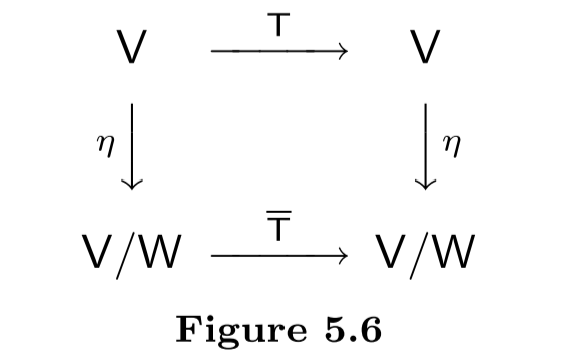
\includegraphics[width=8cm]{images/figure-5-6.png}

\end{exercise}

\begin{proof}
\end{proof}

\begin{exercise} \label{exercise 5.4.28}
Let \(f(t), g(t)\), and \(h(t)\) be the \CPOLY{} of \(\T, \T_W\), and \(\Tover\), respectively.
Prove that \(f(t) = g(t)h(t)\).
Hint: Extend an ordered basis \(\gamma = \{ v_1, v_2, ..., v_k \}\) for \(\W\) to an ordered basis \(\beta = \{ v_1, v_2, ..., v_k, v_{k + 1}, ..., v_n \}\) for \(\V\).
Then show that the \emph{collection of cosets} \(\alpha = \{ v_{k + 1} + \W, v_{k + 2} + \W, ..., v_n + \W \}\) is an ordered basis for \(\V/\W\), and prove that
\[
    [\T]_{\beta} = \begin{pmatrix}
        B_1 & B_2 \\ O B_3
    \end{pmatrix}.
\]
where \(B_1 = [\T_W]_{\gamma}\) and \(B_3 = [\Tover]_{\alpha}\).
\end{exercise}

\begin{proof}
這邊 \(B_1\) equal 的東西感覺有打錯。
\end{proof}

\begin{exercise} \label{exercise 5.4.29}
Use the hint in \EXEC{5.4.28} to prove that if \(\T\) is diagonalizable, then so is \(\Tover\).
\end{exercise}

\begin{proof}
\end{proof}

\begin{exercise} \label{exercise 5.4.30}
Prove that if both \(\T_W\) and \(\Tover\) are diagonalizable and \emph{have no common} eigenvalues, then \(\T\) is diagonalizable.
\end{exercise}

\begin{proof}
\end{proof}

The results of \THM{5.21} and \EXEC{5.4.28} are useful in devising \emph{methods for computing \CPOLY{}s} \textbf{without the use of determinants}.
This is illustrated in the next exercise.

\begin{exercise} \label{exercise 5.4.31}
Let \(A = \begin{pmatrix} 1 & 1 & -3 \\ 2 & 3 & 4 \\ 1 & 2 & 1 \end{pmatrix}\), let \(\T = \LMTRAN_A\), and let \(\W\) the cyclic subspace of \(\SET{R}^3\) generated by \(e_1\).

\begin{enumerate}
\item Use \THM{5.21} to compute the \CPOLY{} of \(\T_W\).
\item Show that \(\{ e_2 + \W \}\) is a basis for \(\SET{R}^3/\W\), and use this fact to compute the \CPOLY{} of \(\T\).
\item Use the results of (a) and (b) to find the \CPOLY{} of \(A\).
\end{enumerate}
\end{exercise}

\begin{proof}
\end{proof}

Exercises 32 through 39 are concerned with direct sums.

\begin{exercise} \label{exercise 5.4.32}
Let \(\T\) be a linear operator on a vector space \(\V\), and let \(\W_1, \W_2 , ..., \W_k\) be \(\T\)-invariant subspaces of \(\V\).
Prove that \(\W_1 + \W_2 + ... + \W_k\) is also a \(\T\)-invariant subspace of \(\V\).
\end{exercise}

\begin{proof}
\end{proof}

\begin{exercise} \label{exercise 5.4.33}
Give a \emph{direct proof} of \THM{5.24} for the case \(k = 2\).
(This result is used in the proof of \THM{5.23}.)
\end{exercise}

\begin{proof}
\end{proof}

\begin{exercise} \label{exercise 5.4.34}
Prove \THM{5.24}.
\emph{Hint}: Begin with \EXEC{5.4.33} and extend it using mathematical induction on \(k\), the number of subspaces.
\end{exercise}

\begin{proof}
\end{proof}

\begin{exercise} \label{exercise 5.4.35}
Let \(\T\) be a linear operator on a finite-dimensional vector space \(\V\).
Prove that \(\T\) is diagonalizable if and only if \(\V\) is the direct sum of \emph{one-dimensional} \(\T\)-invariant subspaces.
\end{exercise}

\begin{proof}
\end{proof}

\begin{exercise} \label{exercise 5.4.36}
Let \(\T\) be a linear operator on a finite-dimensional vector space \(\V\), and let \(\W_1, \W_2, ..., \W_k\) be \(\T\)-invariant subspaces of \(\V\) such that \(v = \W_1 \oplus \W_2 \oplus ... \oplus \W_k\).
Prove that
\[
    \det(\T) = \det(\T_{W_1}) \cdot \det(\T_{W_2}) \cdot \det(\T_{W_k}).
\]
\end{exercise}

\begin{proof}
\end{proof}

\begin{exercise} \label{exercise 5.4.37}
Let \(\T\) be a linear operator on a finite-dimensional vector space \(\V\), and let \(\W_1, \W_2, ..., \W_k\) be \(\T\)-invariant subspaces of \(\V\) such that \(\V = \W_1 \oplus \W_2 \oplus ... \oplus \W_k\).
Prove that \(\T\) is diagonalizable if and only if \(\T_W\), is diagonalizable for all \(i\).
\end{exercise}

\begin{proof}
\end{proof}

\begin{exercise} \label{exercise 5.4.38}
Let \(\mathcal{C}\) be an arbitrary collection of \emph{diagonalizable} linear operators on a finite-dimensional vector space \(\V\).
Prove that there is an ordered basis \(\beta\) such that \([\T]_{\beta}\) is a diagonal matrix for all \(\T \in \mathcal{C}\), if and only if, the operators of \(\mathcal{C}\) commute under composition.
(This is an extension of \EXEC{5.4.25}.)
Hints for the case that the operator commute:
The result is trivial if each operator has only one eigenvalue.
Otherwise, establish the general result by mathematical induction on \(\dim(\V)\), using the fact that \(\V\) is the direct sum of the eigenspaces of some operator in \(\mathcal{C}\) that has more than one eigenvalue.
\end{exercise}

\begin{proof}
\end{proof}

\begin{exercise} \label{exercise 5.4.39}
Let \(B_1, B_2, ..., B_k\) be square matrices with entries in the same field, and let \(A = B_1 \oplus B_2 \oplus ... \oplus B_k\).
Prove that the \CPOLY{} of \(A\) is the product of the \CPOLY{} of the \(B_i\)'s.
\end{exercise}

\begin{proof}
\end{proof}

\begin{exercise} \label{exercise 5.4.40}
Let
\[
    A = \begin{pmatrix}
        1 & 2 & ... & n \\
        n + 1 & n + 2  & ... & 2n \\
        \vdots & \vdots & & \vdots \\
        n^2 - n + 1 & n^2 - n + 2 & ... & n^2
    \end{pmatrix}.
\]
\sloppy Find the \CPOLY{} of \(A\).
\emph{Hint}: First prove that \(A\) has rank \(21\) and that \(\spann(\{ (1, 1, ... , 1), (1, 2, ..., n) \})\) is \(\LMTRAN_A\)-invariant.
\end{exercise}

\begin{proof}
\end{proof}

\begin{exercise} \label{exercise 5.4.41}
Let \(A \in M_{n \X n}(\SET{R})\) be the matrix defined by \(A_{ij} = 1\) for all \(i\) and \(j\).
Find the \CPOLY{} of \(A\).
\end{exercise}

\begin{proof}
\end{proof}